\ifx\wholebook\relax \else
% ------------------------

\documentclass{article}
%------------------- Other types of document example ------------------------
%
%\documentclass[twocolumn]{IEEEtran-new}
%\documentclass[12pt,twoside,draft]{IEEEtran}
%\documentstyle[9pt,twocolumn,technote,twoside]{IEEEtran}
%
%-----------------------------------------------------------------------------
%%
% loading packages
%
\newif\ifpdf
\ifx\pdfoutput\undefined % We're not running pdftex
  \pdffalse
\else
  \pdftrue
\fi
%
%
\ifpdf
  \RequirePackage[pdftex,%
            CJKbookmarks,%
       bookmarksnumbered,%
              colorlinks,%
          linkcolor=blue,%
              hyperindex,%
        plainpages=false,%
       pdfstartview=FitH]{hyperref}
\else
  \RequirePackage[dvipdfm,%
             CJKbookmarks,%
        bookmarksnumbered,%
               colorlinks,%
           linkcolor=blue,%
               hyperindex,%
         plainpages=false,%
        pdfstartview=FitH]{hyperref}
  \AtBeginDvi{\special{pdf:tounicode GBK-EUC-UCS2}} % GBK -> Unicode
\fi
\usepackage{hyperref}

% other packages
%-----------------------------------------------------------------------------
\usepackage{graphicx, color}
\usepackage{CJK}
%
% for programming 
%
\usepackage{verbatim}
\usepackage{listings}


\lstdefinelanguage{Smalltalk}{
  morekeywords={self,super,true,false,nil,thisContext}, % This is overkill
  morestring=[d]',
  morecomment=[s]{"}{"},
  alsoletter={\#:},
  escapechar={!},
  literate=
    {BANG}{!}1
    {UNDERSCORE}{\_}1
    {\\st}{Smalltalk}9 % convenience -- in case \st occurs in code
    % {'}{{\textquotesingle}}1 % replaced by upquote=true in \lstset
    {_}{{$\leftarrow$}}1
    {>>>}{{\sep}}1
    {^}{{$\uparrow$}}1
    {~}{{$\sim$}}1
    {-}{{\sf -\hspace{-0.13em}-}}1  % the goal is to make - the same width as +
    %{+}{\raisebox{0.08ex}{+}}1		% and to raise + off the baseline to match -
    {-->}{{\quad$\longrightarrow$\quad}}3
	, % Don't forget the comma at the end!
  tabsize=2
}[keywords,comments,strings]

\lstloadlanguages{C++, Lisp, Smalltalk}

% ======================================================================

\def\BibTeX{{\rm B\kern-.05em{\sc i\kern-.025em b}\kern-.08em
    T\kern-.1667em\lower.7ex\hbox{E}\kern-.125emX}}

\newtheorem{theorem}{Theorem}

%
% mathematics
%
\newcommand{\be}{\begin{equation}}
\newcommand{\ee}{\end{equation}}
\newcommand{\bmat}[1]{\left( \begin{array}{#1} }
\newcommand{\emat}{\end{array} \right) }
\newcommand{\VEC}[1]{\mbox{\boldmath $#1$}}

% numbered equation array
\newcommand{\bea}{\begin{eqnarray}}
\newcommand{\eea}{\end{eqnarray}}

% equation array not numbered
\newcommand{\bean}{\begin{eqnarray*}}
\newcommand{\eean}{\end{eqnarray*}}

\RequirePackage{CJK,CJKnumb,CJKulem,CJKpunct}
% we use CJK as default environment
\AtBeginDocument{\begin{CJK*}{GBK}{song}\CJKtilde\CJKindent\CJKcaption{GB}}
\AtEndDocument{\clearpage\end{CJK*}}

%
% loading packages
%
\newif\ifpdf
\ifx\pdfoutput\undefined % We're not running pdftex
  \pdffalse
\else
  \pdftrue
\fi
%
%
\ifpdf
  \RequirePackage[pdftex,%
       bookmarksnumbered,%
              colorlinks,%
          linkcolor=blue,%
              hyperindex,%
        plainpages=false,%
       pdfstartview=FitH]{hyperref}
\else
  \RequirePackage[dvipdfm,%
        bookmarksnumbered,%
               colorlinks,%
           linkcolor=blue,%
               hyperindex,%
         plainpages=false,%
        pdfstartview=FitH]{hyperref}
\fi
\usepackage{hyperref}

% other packages
%-----------------------------------------------------------------------------
\usepackage{graphicx, color}
%
% for programming 
%
\usepackage{verbatim}
\usepackage{listings}
\usepackage{algorithmic} %for pseudocode
\usepackage{algorithm}


\lstdefinelanguage{Smalltalk}{
  morekeywords={self,super,true,false,nil,thisContext}, % This is overkill
  morestring=[d]',
  morecomment=[s]{"}{"},
  alsoletter={\#:},
  escapechar={!},
  literate=
    {BANG}{!}1
    {UNDERSCORE}{\_}1
    {\\st}{Smalltalk}9 % convenience -- in case \st occurs in code
    % {'}{{\textquotesingle}}1 % replaced by upquote=true in \lstset
    {_}{{$\leftarrow$}}1
    {>>>}{{\sep}}1
    {^}{{$\uparrow$}}1
    {~}{{$\sim$}}1
    {-}{{\sf -\hspace{-0.13em}-}}1  % the goal is to make - the same width as +
    %{+}{\raisebox{0.08ex}{+}}1		% and to raise + off the baseline to match -
    {-->}{{\quad$\longrightarrow$\quad}}3
	, % Don't forget the comma at the end!
  tabsize=2
}[keywords,comments,strings]

\lstloadlanguages{C++, Lisp, Haskell, Python, Smalltalk}

% ======================================================================

\def\BibTeX{{\rm B\kern-.05em{\sc i\kern-.025em b}\kern-.08em
    T\kern-.1667em\lower.7ex\hbox{E}\kern-.125emX}}

\newtheorem{theorem}{Theorem}

%
% mathematics
%
\newcommand{\be}{\begin{equation}}
\newcommand{\ee}{\end{equation}}
\newcommand{\bmat}[1]{\left( \begin{array}{#1} }
\newcommand{\emat}{\end{array} \right) }
\newcommand{\VEC}[1]{\mbox{\boldmath $#1$}}

% numbered equation array
\newcommand{\bea}{\begin{eqnarray}}
\newcommand{\eea}{\end{eqnarray}}

% equation array not numbered
\newcommand{\bean}{\begin{eqnarray*}}
\newcommand{\eean}{\end{eqnarray*}}




\setcounter{page}{1}

\begin{document}

%--------------------------

% ================================================================
%                 COVER PAGE
% ================================================================

\title{B-Trees}

\author{Larry~LIU~Xinyu
\thanks{{\bfseries Larry LIU Xinyu } \newline
  Email: liuxinyu95@gmail.com \newline}
  }

\maketitle
\fi

\markboth{B-Trees}{Elementary Algorithms}

\ifx\wholebook\relax
\chapter{B-Trees}
\numberwithin{Exercise}{chapter}
\fi

%{\bfseries Corresponding Author:} Larry LIU Xinyu

% ================================================================
%                 Introduction
% ================================================================
\section{Introduction}
\index{B-tree}
\label{introduction}

B-Tree is important data structure.
It is widely used in modern file systems. Some
are implemented based on B+ tree, which is extended from B-tree.
B-tree is also widely used in database systems.

Some textbooks introduce B-tree with the the problem of how to access a
large block of data on magnetic disks or secondary storage devices\cite{CLRS}.
It is also helpful to understand B-tree as a generalization of balanced binary
search tree\cite{wiki-b-tree}.

Refer to the Figure \ref{fig:btree-example}, It is easy to find the difference
and similarity of B-tree regarding to binary search tree.

\begin{figure}[htbp]
   \begin{center}
	\includegraphics[scale=0.5]{img/btree-example.ps}
   \caption{Example B-Tree} \label{fig:btree-example}
   \end{center}
\end{figure}

Remind the definition of binary search tree. A binary search tree is
\begin{itemize}
\item either an empty node;
\item or a node contains 3 parts, a value, a left child and a right child.
Both children are also binary search trees.
\end{itemize}

The binary search tree satisfies the constraint that.
\begin{itemize}
\item all the values on the left child are not greater than the value of of this node;
\item the value of this node is not greater than any values on the right child.
\end{itemize}

For non-empty binary tree $(L, k, R)$, where $L$, $R$ and $k$
are the left, right children, and the key. Function $Key(T)$ accesses
the key of tree $T$.
The constraint can be represented as the following.

\begin{equation}
\forall x \in L, \forall y \in R \\
\Rightarrow Key(x) \leq k \leq Key(y)
\end{equation}

If we extend this definition to allow multiple keys and children, we get the
B-tree definition.

A B-tree
\begin{itemize}
\item is either empty;
\item or contains $n$ keys, and $n+1$ children, each child is
also a B-Tree, we denote these keys and children as $k_1, k_2, ..., k_n$
and $c_1, c_2, ..., c_n, c_{n+1}$.
\end{itemize}

Figure \ref{fig:btree-node} illustrates a B-Tree node.

\begin{figure}[htbp]
  \centering
	\includegraphics[scale=0.5]{img/btree-node.ps}
  \caption{A B-Tree node} \label{fig:btree-node}
\end{figure}

The keys and children in a node satisfy the following order constraints.

\begin{itemize}
\item Keys are stored in non-decreasing order. that $k_1 \leq k_2 \leq ... \leq k_n$;
\item for each $k_i$, all elements stored in child $c_i$ are not greater
than $k_i$, while $k_i$ is not greater than any values stored in child $c_{i+1}$.
\end{itemize}

The constraints can be represented as in equation (\ref{eq:btree-order})
as well.

\begin{equation}
\forall x_i \in c_i, i=0, 1, ..., n, \Rightarrow x_1 \leq k_1 \leq
x_2 \leq k_2 \leq ... \leq x_n \leq k_n \leq x_{n+1}
\label{eq:btree-order}
\end{equation}

Finally, after adding some constraints to make the tree balanced, we get the
complete B-tree definition.

\begin{itemize}
\item All leaves have the same depth;
\item We define integral number, $t$, as the {\em minimum degree} of
B-tree;
    \begin{itemize}
        \item each node can have at most $2t-1$ keys;
        \item each node can have at least $t-1$ keys, except the root;
    \end{itemize}
\end{itemize}

Consider a B-tree holds $n$ keys. The minimum degree $t \geq 2$.
The height is $h$. All the nodes have at least $t-1$ keys except the
root. The root contains at least 1 key. There are at least 2 nodes
at depth 1, at least $2t$ nodes at depth 2, at least $2t^2$ nodes
at depth 3, ..., finally, there are at least $2t^{h-1}$ nodes at
depth $h$. Times all nodes with $t-1$ except for root,
the total number of keys satisfies the following inequality.

\be
\begin{array}{rl}
n & \geq 1 + (t-1)(2 + 2t + 2t^2 + ... + 2t^{h-1}) \\
  & = 1 + 2(t-1) \displaystyle \sum_{k=0}^{h-1} t^k \\
  & = 1 + 2(t-1) \displaystyle \frac{t^h-1}{t-1} \\
  & = 2t^h - 1
\end{array}
\ee

Thus we have the inequality between the height and the number
of keys.

\be
h \leq \log_t \frac{n+1}{2}
\ee

This is the reason why B-tree is balanced. The simplest B-tree
is so called 2-3-4 tree, where $t=2$, that every node except
root contains 2 or 3 or 4 keys. red-black tree can be mapped
to 2-3-4 tree essentially.

The following Python code shows example B-tree definition.
It explicitly pass $t$ when create a node.

\lstset{language=Python}
\begin{lstlisting}
class BTree:
    def __init__(self, t):
        self.t = t
        self.keys = []
        self.children = []
\end{lstlisting}

B-tree nodes commonly have satellite data as well. We ignore
satellite data for illustration purpose.

In this chapter, we will firstly introduce how to generate B-tree by insertion.
Two different methods will be explained. One is the classic method
as in \cite{CLRS}, that we split the node before insertion if it's full;
the other is the modify-fix approach which is quite similar to the
red-black tree solution \cite{okasaki-rbtree} \cite{wiki-b-tree}.
We will next explain how to delete
key from B-tree and how to look up a key.


% ================================================================
%                 Insertion
% ================================================================
\section{Insertion}
\index{B-tree!insert}
\label{btree-insertion}

B-tree can be created by inserting
keys repeatedly. The basic idea is similar to the binary
search tree. When insert key $x$, from the tree root, we examine all the
keys in the node to find a position where all the keys on the left are
less than $x$, while all the keys on the right are greater than $x$.\footnote{This is a strong constraint. In fact, only less-than and equality testing is neccessary. The later exercise address this point.}
If the current node is a leaf node, and it is not full (there are
less then $2t-1$ keys in this node), $x$ will be insert at this position.
Otherwise, the position points to a child node.
We need recursively insert $x$ to it.

\begin{figure}[htbp]
  \centering
  \subfloat[Insert key 22 to the 2-3-4 tree. $22 > 20$, go to the right child; $22 < 26$ go to the first child.]{\includegraphics[scale=0.5]{img/btree-insert-simple1.ps}} \\
  \subfloat[$21 < 22 < 25$, and the leaf isn't full.]{\includegraphics[scale=0.5]{img/btree-insert-simple2.ps}}
  \caption{Insertion is similar to binary search tree.} \label{fig:btree-insert-simple}
\end{figure}

Figure \ref{fig:btree-insert-simple} shows one example. The B-tree illustrated
is 2-3-4 tree. When insert key $x=22$, because it's greater than the root,
the right child contains key 26, 38, 45 is examined next; Since $22 < 26$,
the first child contains key 21 and 25 are examined. This is a leaf
node, and it is not full, key 22 is inserted to this node.

However, if there are $2t-1$ keys in the leaf, the new key $x$ can't
be inserted, because this node is 'full'. When try to insert key 18
to the above example B-tree will meet this problem. There are 2 methods to
solve it.

%=========================================================================
%       Splitting
%=========================================================================
\subsection{Splitting}
\index{B-tree!split}
\label{split}

\subsubsection{Split before insertion}

If the node is full, one method to solve the problem is to
split to node before insertion.

For a node with $t-1$ keys, it can be divided into 3 parts as shown in
Figure \ref{fig:node-split}. the left part contains the first $t-1$ keys
and $t$ children. The right part contains the rest $t-1$ keys
and $t$ children. Both left part and right part are valid B-tree
nodes. the middle part is the $t$-th key. We can push it up
to the parent node (if the current node is root, then the this key,
with the two children will be the new root).

\begin{figure}[htbp]
  \centering
  \subfloat[Before split]{\includegraphics[scale=0.5]{img/split-node-before.ps}} \\
  \subfloat[After split]{\includegraphics[scale=0.5]{img/split-node-after.ps}}
  \caption{Split node}
  \label{fig:node-split}
\end{figure}

For node $x$, denote $K(x)$
as keys, $C(x)$ as children. The $i$-th key as $k_i(x)$, the $j$-th child
as $c_j(x)$. Below algorithm describes how to split the $i$-th child for a given node.

\begin{algorithmic}[1]
\Procedure{Split-Child}{$node, i$}
  \State $x \gets c_i(node)$
  \State $y \gets$ \Call{CREATE-NODE}{}
  \State \Call{Insert}{$K(node), i, k_t(x)$}
  \State \Call{Insert}{$C(node), i + 1, y$}
  \State $K(y) \gets \{k_{t+1}(x), k_{t+2}(x), ..., k_{2t-1}(x)\}$
  \State $K(x) \gets \{k_1(x), k_2(x), ..., k_{t-1}(x)\}$
  \If{$y$ is not leaf}
    \State $C(y) \gets \{c_{t+1}(x), c_{t+2}(x), ..., c_{2t}(x)\}$
    \State $C(x) \gets \{c_1(x), c_2(x), ..., c_t(x)\}$
  \EndIf
\EndProcedure
\end{algorithmic}

The following example Python program implements this child splitting algorithm.

\lstset{language=Python}
\begin{lstlisting}
def split_child(node, i):
    t = node.t
    x = node.children[i]
    y = BTree(t)
    node.keys.insert(i, x.keys[t-1])
    node.children.insert(i+1, y)
    y.keys = x.keys[t:]
    x.keys = x.keys[:t-1]
    if not is_leaf(x):
        y.children = x.children[t:]
        x.children = x.children[:t]
\end{lstlisting}

Where function \texttt{is\_leaf} test if a node is leaf.

\lstset{language=Python}
\begin{lstlisting}
def is_leaf(t):
    return t.children == []
\end{lstlisting}

%=========================================================================
%       Split before insertion
%=========================================================================

After splitting, a key is pushed up to its parent node.
It is quite possible that the parent node has already been full.
And this pushing violates the B-tree property.

In order to solve this problem, we can check from the root along
the path of insertion traversing till the leaf. If there is any node
in this path is full, the splitting is applied. Since the parent
of this node has been examined, it is ensured that there are
less than $2t-1$ keys in the parent. It won't make the
parent full if pushing up one key. This approach only need one single
pass down the tree without any back-tracking.

If the root need splitting, a new node is created as the new root.
There is no keys in this new created root, and the previous root is
set as the only child. After that, splitting is performed top-down.
And we can insert the new key finally.

\begin{algorithmic}[1]
\Function{Insert}{$T, k$}
  \State $r \gets T$
  \If{$r$ is full} \Comment{root is full}
    \State $s \gets$ \Call{CREATE-NODE}{}
    \State $C(s) \gets \{r\}$
    \State \Call{Split-Child}{$s, 1$}
    \State $r \gets s$
  \EndIf
  \State \Return \Call{Insert-Nonfull}{$r, k$}
\EndFunction
\end{algorithmic}

Where algorithm \textproc{Insert-Nonfull} assumes the node passed in
is not full. If it is a leaf node, the new key is inserted to
the proper position based on the order; Otherwise, the algorithm
finds a proper child node to which the new key will be inserted.
If this child is full, splitting will be performed.

\begin{algorithmic}[1]
\Function{Insert-Nonfull}{$T, k$}
  \If{$T$ is leaf}
    \State $i \gets 1$
    \While{$i \leq |K(T)| \land k > k_i(T)$}
      \State $i \gets i+1$
    \EndWhile
    \State \Call{Insert}{$K(T), i, k$}
  \Else
    \State $i \gets |K(T)|$
    \While{$i>1 \land k < k_i(T)$}
      \State $i \gets i-1$
    \EndWhile
    \If{$c_i(T)$ is full}
      \State \Call{Split-Child}{$T, i$}
      \If{$k > k_i(T)$}
        \State $i \gets i+1$
      \EndIf
    \EndIf
    \State \Call{Insert-Nonfull}{$c_i(T), k$}
  \EndIf
  \State \Return $T$
\EndFunction
\end{algorithmic}

This algorithm is recursive. In B-tree,
the minimum degree $t$ is typically relative to magnetic disk structure.
Even small depth can support huge amount of data
(with $t=10$, maximum to 10 billion data can be stored in a B-tree with height of 10).
The recursion can also be eliminated. This is left as exercise to the reader.

Figure \ref{fig:btree-insert} shows the result of continuously inserting
keys G, M, P, X, A, C, D, E, J, K, N, O, R, S, T, U, V, Y, Z to the empty tree.
The first result is the 2-3-4 tree ($t=2$). The second result shows how
it varies when $t=3$.

\begin{figure}[htbp]
  \centering
  \subfloat[2-3-4 tree.]{\includegraphics[scale=0.5]{img/btree-insert-2-3-4.ps}}\\
  \subfloat[$t=3$]{\includegraphics[scale=0.5]{img/btree-insert-3.ps}}
  \caption{Insertion result} \label{fig:btree-insert}
\end{figure}

Below example Python program implements this algorithm.
\lstset{language=Python}
\begin{lstlisting}
def insert(tr, key):
    root = tr
    if is_full(root):
        s = BTree(root.t)
        s.children.insert(0, root)
        split_child(s, 0)
        root = s
    return insert_nonfull(root, key)
\end{lstlisting}

And the insertion to non-full node is implemented as the following.

\begin{lstlisting}
def insert_nonfull(tr, key):
    if is_leaf(tr):
        ordered_insert(tr.keys, key)
    else:
        i = len(tr.keys)
        while i>0 and key < tr.keys[i-1]:
            i = i-1
        if is_full(tr.children[i]):
            split_child(tr, i)
            if key>tr.keys[i]:
                i = i+1
        insert_nonfull(tr.children[i], key)
    return tr
\end{lstlisting}

Where function \texttt{ordered\_insert} is used to insert an element
to an ordered list. Function \texttt{is\_full} tests if a node contains
$2t-1$ keys.

\begin{lstlisting}
def ordered_insert(lst, x):
    i = len(lst)
    lst.append(x)
    while i>0 and lst[i]<lst[i-1]:
        (lst[i-1], lst[i]) = (lst[i], lst[i-1])
        i=i-1

def is_full(node):
    return len(node.keys) >= 2 * node.t - 1
\end{lstlisting}

For the array based collection, append on the tail is much more effective than
insert in other position, because the later takes $O(n)$ time, if the length
of the collection is $n$. The \texttt{ordered\_insert} program firstly appends
 the new element at the end of the existing collection, then iterates from the
last element to the first one, and checks if the current two elements next to each other
are ordered. If not, these two elements will be swapped.

% ================================================================
%               Insert and fix method
% ================================================================

\subsubsection{Insert then fixing}

In functional settings, B-tree insertion can be realized in a way similar to
red-black tree. When insert a key to red-black tree, it is firstly inserted
as in the normal binary search tree, then recursive fixing is performed to
resume the balance of the tree. B-tree can be viewed as extension to the
binary search tree, that each node contains multiple keys and children.
We can firstly insert the key without considering if the node is full.
Then perform fixing to satisfy the minimum degree constraint.

\be
insert(T, k) = fix(ins(T, k))
\ee

Function $ins(T, k)$ traverse the B-tree $T$ from root to find a proper
position where key $k$ can be inserted. After that, function $fix$ is
applied to resume the B-tree properties. Denote B-tree in a form of
$T = (K, C, t)$, where $K$ represents keys, $C$ represents children,
and $t$ is the minimum degree.

Below is the Haskell definition of B-tree.

\lstset{language=Haskell}
\begin{lstlisting}
data BTree a = Node{ keys :: [a]
                   , children :: [BTree a]
                   , degree :: Int} deriving (Eq)
\end{lstlisting}

The insertion function can be provided based on this definition.

\lstset{language=Haskell}
\begin{lstlisting}
insert tr x = fixRoot $ ins tr x
\end{lstlisting} %$

There are two cases when realize $ins(T, k)$ function. If the tree $T$ is
leaf, $k$ is inserted to the keys; Otherwise if $T$ is the branch node, we
need recursively insert $k$ to the proper child.

Figure \ref{fig:recursive-insert} shows the branch case. The
algorithm first locates the position. for certain key $k_i$,
if the new key $k$ to be inserted satisfy $k_{i-1}<k<k_i$,
Then we need recursively insert $k$ to child $c_i$.

This position divides the node into 3 parts, the left part,
the child $c_i$ and the right part.

\begin{figure}[htbp]
  \centering
  \subfloat[Locate the child to insert.]{\includegraphics[scale=0.5]{img/insert-before.ps}} \\
  \subfloat[Recursive insert.]{\includegraphics[scale=0.5]{img/insert-after.ps}}
  \caption{Insert a key to a branch node} \label{fig:recursive-insert}
\end{figure}

\be
ins(T, k) = \left \{
  \begin{array}
  {r@{\quad:\quad}l}
  (K' \cup \{k\} \cup K'', \phi, t) & C = \phi, (K', K'') = divide(K, k) \\
  make((K', C_1), ins(c, k), (K'', C_2')) & (C_1, C_2) = split(|K'|, C)
  \end{array}
\right.
\ee

The first clause deals with the leaf case.
Function $divide(K, k)$ divide keys into two parts, all keys in the first
part are not greater than $k$, and all rest keys are not less than $k$.

\[
K = K' \cup K'' \land \forall k' \in K, k'' \in K'' \Rightarrow k' \leq k \leq k''
\]

The second clause handle the branch case.
Function $split(n, C)$ splits children in two parts, $C_1$ and $C_2$.
$C_1$ contains the first $n$ children; and $C_2$ contains the rest.
Among $C_2$, the first child is denoted as $c$, and others are
represented as $C_2'$.

Here the key $k$ need be recursively inserted into child $c$. Function
$make$ takes 3 parameter. The first and the third are pairs of
key and children; the second parameter is a child node. It examines
if a B-tree node made from these keys and children violates the
minimum degree constraint and performs fixing if necessary.

\be
make((K', C'), c, (K'', C'')) = \left \{
  \begin{array}
  {r@{\quad:\quad}l}
  fixFull((K', C'), c, (K'', C'')) & full(c) \\
  (K' \cup K'', C' \cup \{c\} \cup C'', t) & otherwise
  \end{array}
\right.
\ee

Where function $full(c)$ tests if the child $c$ is full.
Function $fixFull$ splits the the child $c$, and forms a new B-tree node
with the pushed up key.

\be
fixFull((K', C'), c, (K'', C'')) = (K' \cup \{k'\} \cup K'', C' \cup \{c_1, c_2\} \cup C'', t)
\ee

Where $(c_1, k', c_2) = split(c)$. During splitting, the first $t-1$ keys and $t$ children
are extract to one new child, the last $t-1$ keys and $t$ children form another child.
The $t$-th key $k'$ is pushed up.

With all the above functions defined, we can realize $fix(T)$ to complete the functional B-tree
insertion algorithm. It firstly checks if the root contains too
many keys. If it exceeds the limit, splitting will be applied.
The split result will be used to make a new node, so the total
height of the tree increases by one.

\be
fix(T) = \left \{
  \begin{array}
  {r@{\quad:\quad}l}
  c & T = (\phi, \{c\}, t) \\
  (\{k'\}, \{c_1, c_2\}, t) & full(T), (c_1, k', c_2) = split(T) \\
  T & otherwise
  \end{array}
\right.
\ee

The following Haskell example code implements the B-tree insertion.

\lstset{language=Haskell}
\begin{lstlisting}
import qualified Data.List as L

ins (Node ks [] t) x = Node (L.insert x ks) [] t
ins (Node ks cs t) x = make (ks', cs') (ins c x) (ks'', cs'')
    where
      (ks', ks'') = L.partition (<x) ks
      (cs', (c:cs'')) = L.splitAt (length ks') cs

fixRoot (Node [] [tr] _) = tr -- shrink height
fixRoot tr = if full tr then Node [k] [c1, c2] (degree tr)
             else tr
    where
      (c1, k, c2) = split tr

make (ks', cs') c (ks'', cs'')
    | full c = fixFull (ks', cs') c (ks'', cs'')
    | otherwise = Node (ks'++ks'') (cs'++[c]++cs'') (degree c)

fixFull (ks', cs') c (ks'', cs'') = Node (ks'++[k]++ks'')
                                         (cs'++[c1,c2]++cs'') (degree c)
    where
      (c1, k, c2) = split c

full tr = (length $ keys tr) > 2*(degree tr)-1
\end{lstlisting}

Figure \ref{fig:btree-insert-fp} shows the varies of results of building B-trees
by continuously inserting keys "GMPXACDEJKNORSTUVYZ".

\begin{figure}[htbp]
  \centering
  \subfloat[Insert result of a 2-3-4 tree.]{\includegraphics[scale=0.5]{img/btree-insert-fp-234.ps}} \\
  \subfloat[Insert result of a B-tree with $t = 3$]{\includegraphics[scale=0.5]{img/btree-insert-fp-3.ps}}
    \caption{Insert then fixing results} \label{fig:btree-insert-fp}
\end{figure}

Compare to the imperative insertion result
as shown in figure \ref{fig:btree-insert-fp}
we can found that there are different. However, they are all valid
because all B-tree properties
are satisfied.


% ================================================================
%               Deletion
% ================================================================
\section{Deletion}
\index{B-tree!delete}

Deleting a key from
B-tree may violate balance properties. Except the root, a node shouldn't
contain too few keys less than $t-1$, where $t$ is the
minimum degree.

Similar to the approaches for insertion, we can either do some preparation
so that the node from where the key being deleted contains enough
keys; or do some fixing after the deletion if the node has too few keys.


% ================================================================
%               Merge before delete method
% ================================================================
\subsection{Merge before delete method}

We start from the easiest case. If the key $k$ to be deleted
can be located in node $x$, and $x$ is a leaf node,
we can directly remove $k$ from $x$. If $x$ is the root (the only
node of the tree), we needn't worry about there are too few
keys after deletion. This case is named as case 1 later.

In most cases, we start from the root, along a path to locate
where is the node contains $k$. If $k$ can be located in the
internal node $x$, there are three sub cases.

\begin{itemize}
\item Case 2a, If the child $y$ precedes $k$ contains enough keys (more than $t$),
we replace $k$ in node $x$ with $k'$, which is
the predecessor of $k$ in child $y$. And recursively remove $k'$
from $y$.

The predecessor of $k$ can be easily located as the last key of child
$y$.

This is shown in figure \ref{fig:btree-del-case2a}.

\begin{figure}[htbp]
  \centering
    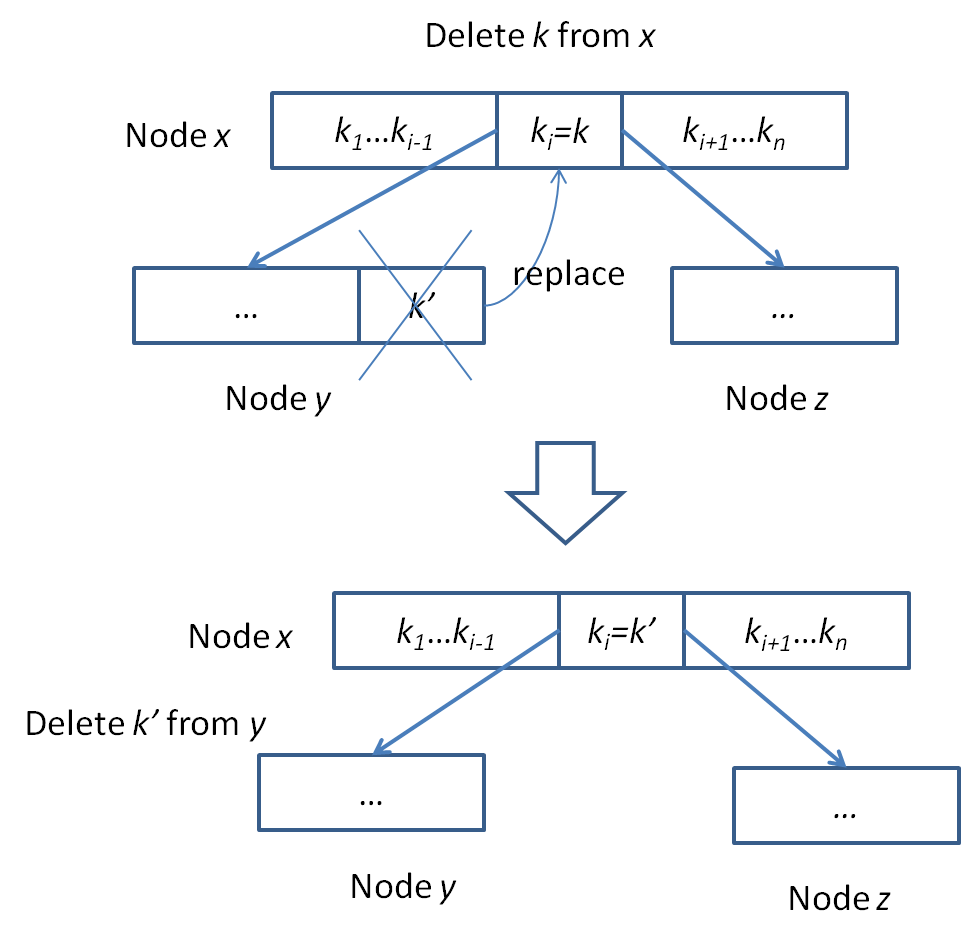
\includegraphics[scale=0.5]{img/btree-del-case2a.eps}
    \caption{Replace and delete from predecessor.} \label{fig:btree-del-case2a}
\end{figure}

\item Case 2b, If $y$ doesn't contain enough keys, while the child $z$
follows $k$ contains more than $t$ keys. We replace $k$ in node $x$
with $k''$, which is the successor of $k$ in child $z$. And recursively
remove $k''$ from $z$.

The successor of $k$ can be easily located as the first key of child $z$.

This sub-case is illustrated in figure \ref{fig:btree-del-case2b}.

\begin{figure}[htbp]
  \centering
    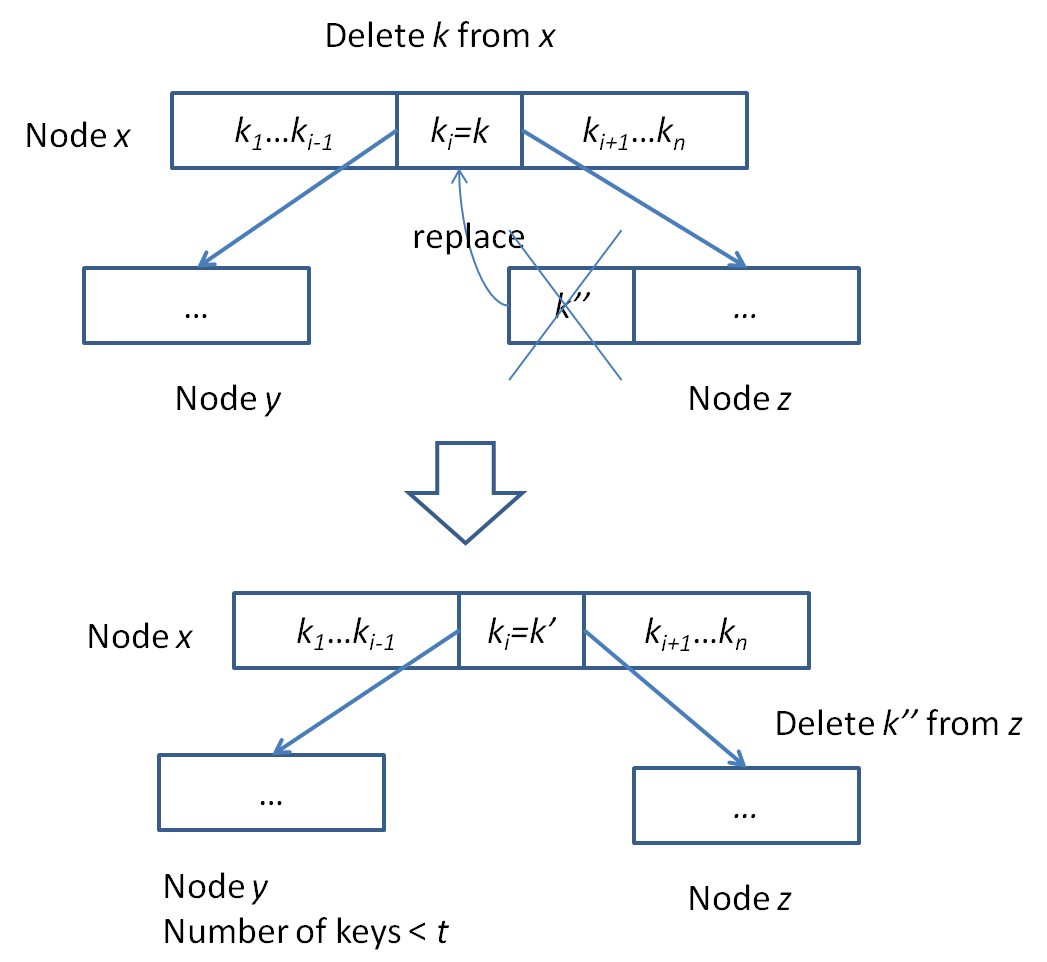
\includegraphics[scale=0.5]{img/btree-del-case2b.eps}
    \caption{Replace and delete from successor.} \label{fig:btree-del-case2b}
\end{figure}

\item Case 2c, Otherwise, if neither $y$, nor $z$ contains enough keys, we
can merge $y$, $k$ and $z$ into one new node, so that this new node
contains $2t-1$ keys. After that, we can then recursively do the removing.

Note that after merge, if the current node doesn't contain any keys,
which means $k$ is the only key in $x$. $y$ and $z$ are the only two
children of $x$. we need shrink the tree height by one.
\end{itemize}

Figure \ref{fig:btree-del-case2c} illustrates this sub-case.

\begin{figure}[htbp]
  \centering
    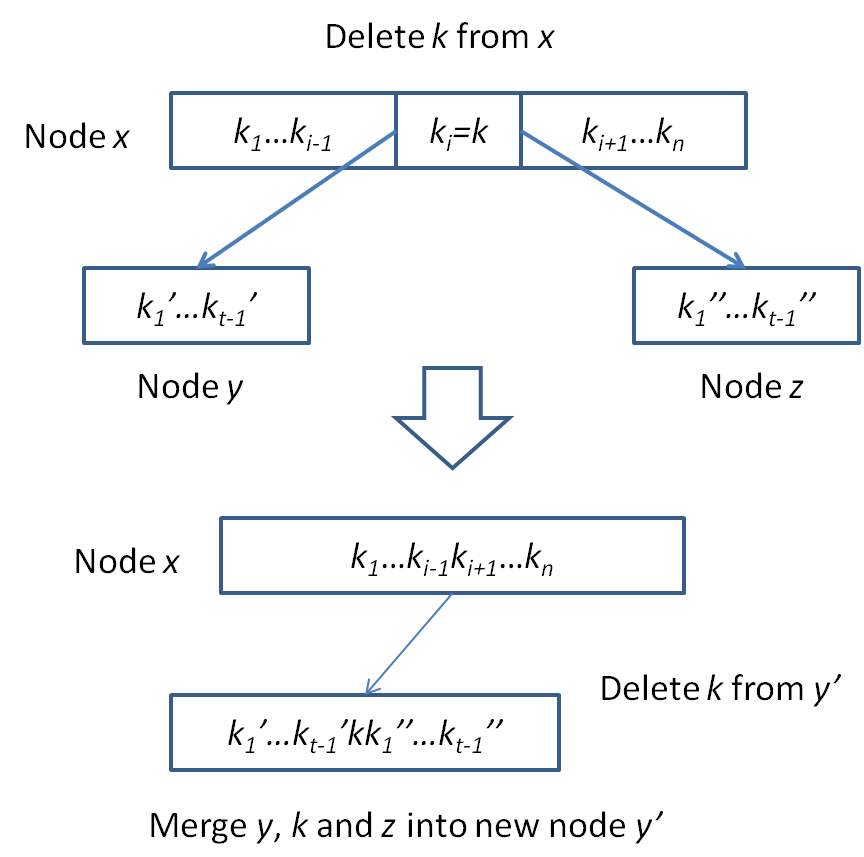
\includegraphics[scale=0.5]{img/btree-del-case2c.eps}
    \caption{Merge and delete.} \label{fig:btree-del-case2c}
\end{figure}

the last case states that, if $k$ can't be located in node $x$, the algorithm
need find a child node $c_i$ in $x$, so that the sub-tree $c_i$
contains $k$. Before the deletion is recursively applied in $c_i$, we
need make sure that there are at least $t$ keys in $c_i$. If there are
not enough keys, the following adjustment is performed.

\begin{itemize}
\item Case 3a, We check the two sibling of $c_i$, which are $c_{i-1}$ and $c_{i+1}$.
If either one contains enough keys (at least $t$ keys), we move
one key from $x$ down to $c_i$, and move one key from the sibling up to
$x$. Also we need move the relative child from the sibling to $c_i$.

This operation makes $c_i$ contains enough keys for deletion. we can
next try to delete $k$ from $c_i$ recursively.

Figure \ref{fig:btree-del-case3a} illustrates this case.

\begin{figure}[htbp]
  \centering
    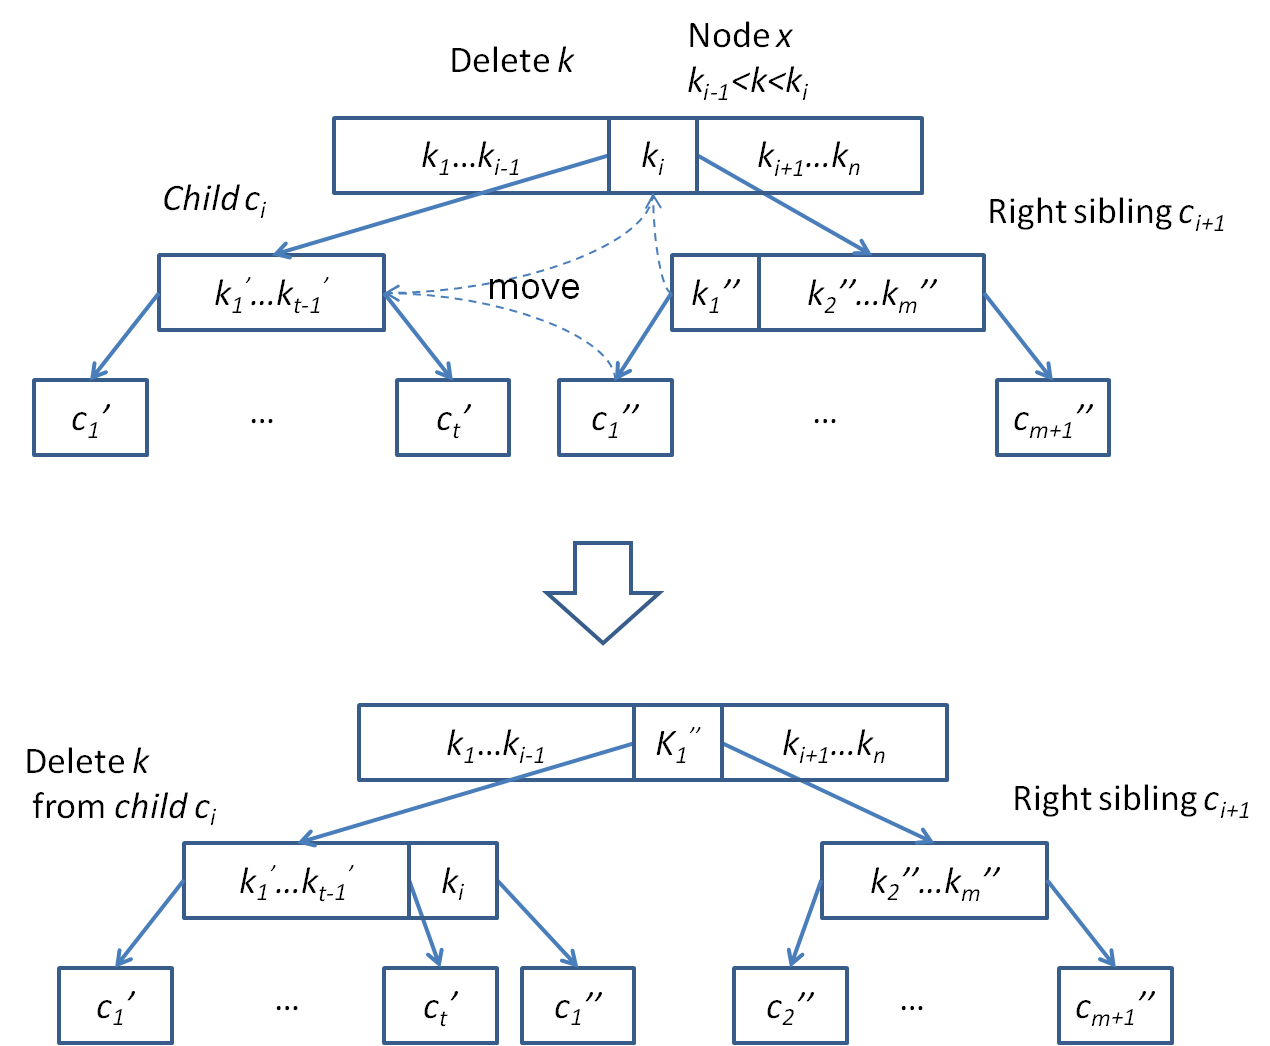
\includegraphics[scale=0.5]{img/btree-del-case3a.eps}
    \caption{Borrow from the right sibling.}
    \label{fig:btree-del-case3a}
\end{figure}

\item Case 3b, In case neither one of the two siblings contains enough keys, we then
merge $c_i$, a key from $x$, and either one of the sibling into a new
node. Then do the deletion on this new node.
\end{itemize}

Figure \ref{fig:btree-del-case3b} shows this case.

\begin{figure}[htbp]
  \centering
    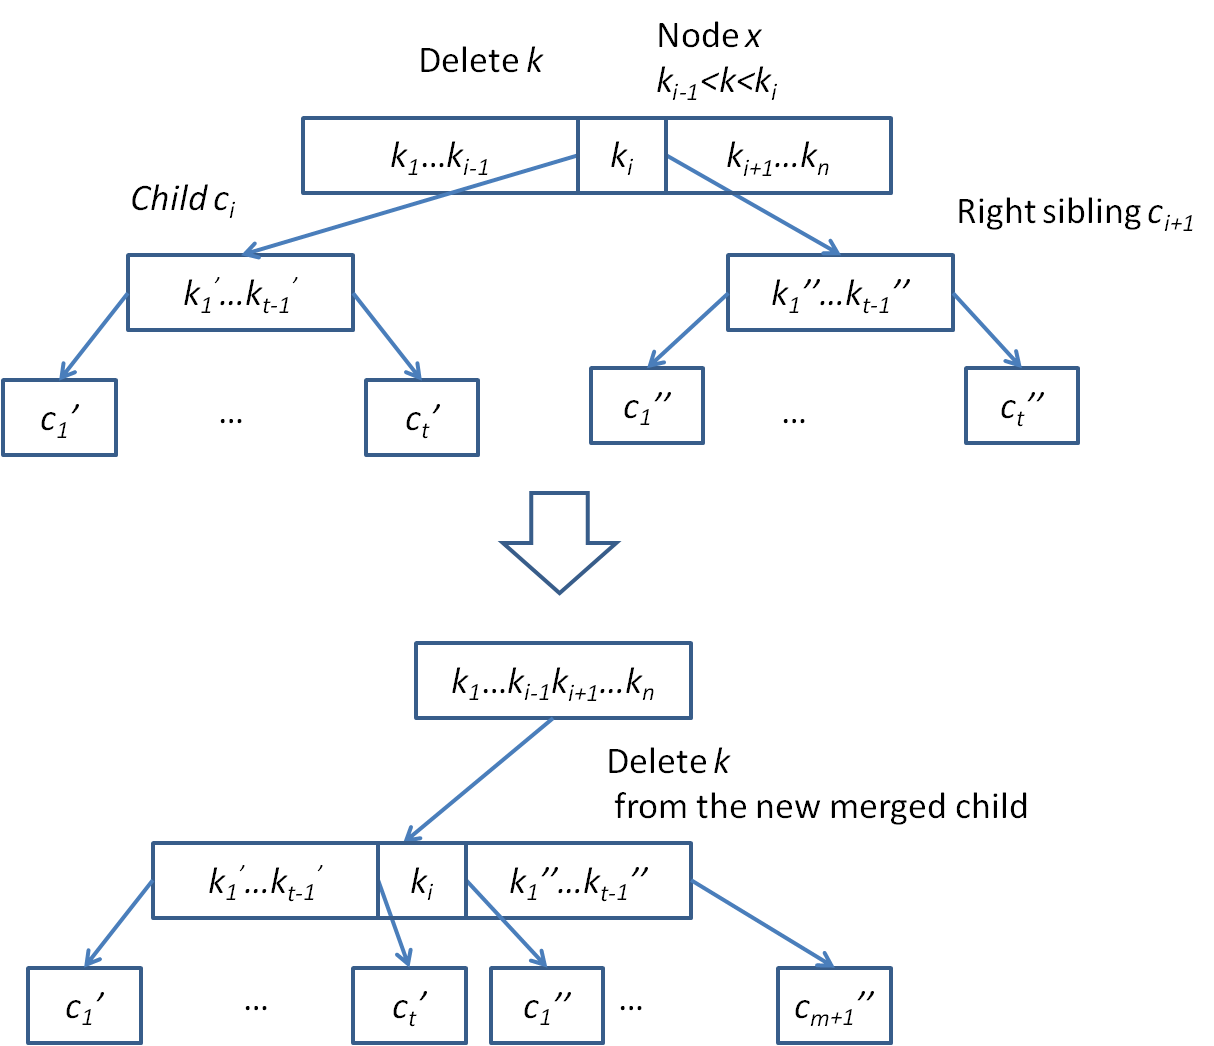
\includegraphics[scale=0.5]{img/btree-del-case3b.eps}
    \caption{Merge $c_i$, $k$, and $c_{i+1}$ to a new node.}
    \label{fig:btree-del-case3b}
\end{figure}

Before define the B-tree delete algorithm, we need provide some auxiliary
functions. Function \textproc{Can-Del} tests if a node contains enough keys
for deletion.

\begin{algorithmic}[1]
\Function{Can-Del}{$T$}
  \State \Return $|K(T)| \ge t$
\EndFunction
\end{algorithmic}

Procedure \textproc{Merge-Children}($T, i$) merges child $c_i(T)$, key $k_i(T)$,
and child $c_{i+1}(T)$ into one big node.

\begin{algorithmic}[1]
\Procedure{Merge-Children}{$T, i$} \Comment{Merge $c_i(T)$, $k_i(T)$, and $c_{i+1}(T)$}
  \State $x \gets c_i(T)$
  \State $y \gets c_{i+1}(T)$
  \State $K(x) \gets K(x) \cup \{k_i(T)\} \cup K(y)$
  \State $C(x) \gets C(x) \cup C(y)$
  \State \Call{Remove-At}{$K(T), i$}
  \State \Call{Remove-At}{$C(T), i+1$}
\EndProcedure
\end{algorithmic}

Procedure \textproc{Merge-Children} merges the $i$-th child, the $i$-th key,
and $i+1$-th child of node $T$ into a new child, and remove the
$i$-th key and $i+1$-th child from $T$ after merging.

With these functions defined, the B-tree deletion algorithm can be given by
realizing the above 3 cases.

\begin{algorithmic}[1]
\Function{Delete}{$T, k$}
  \State $i \gets 1$
  \While{$i \leq |K(T)|$}
    \If{$k = k_i(T)$}
      \If{$T$ is leaf} \Comment{case 1}
        \State \Call{Remove}{$K(T), k$}
      \Else \Comment{case 2}
        \If{\Call{Can-Del}{$c_i(T)$}} \Comment{case 2a}
          \State $k_i(T) \gets$ \Call{Last-Key}{$c_i(T)$}
          \State \Call{Delete}{$c_i(T), k_i(T)$}
        \ElsIf{\Call{Can-Del}{$c_{i+1}(T)$}} \Comment{case 2b}
          \State $k_i(T) \gets$ \Call{First-Key}{$c_{i+1}(T)$}
          \State \Call{Delete}{$c_{i+1}(T), k_i(T)$}
        \Else \Comment{case 2c}
          \State \Call{Merge-Children}{$T, i$}
          \State \Call{Delete}{$c_i(T), k$}
          \If{$K(T) = NIL$}
            \State $T \gets c_i(T)$ \Comment{Shrinks height}
          \EndIf
        \EndIf
      \EndIf
      \State \Return $T$
    \ElsIf{$k < k_i(T)$}
      \State Break
    \Else
      \State $i \gets i+1$
    \EndIf
  \EndWhile
  \Statex
  \If{$T$ is leaf}
    \State \Return $T$ \Comment{$k$ doesn't exist in $T$.}
  \EndIf
  \If{$\lnot$ \Call{Can-Del}{$c_i(T)$}}  \Comment{case 3}
    \If{$i>1 \land$ \Call{Can-Del}{$c_{i-1}(T)$}} \Comment{case 3a: left sibling}
      \State \Call{Insert}{$K(c_i(T)), k_{i-1}(T)$}
      \State $k_{i-1}(T) \gets$ \Call{Pop-Back}{$K(c_{i-1}(T))$}
      \If{$c_i(T)$ isn't leaf}
        \State $c \gets$ \Call{Pop-Back}{$C(c_{i-1}(T))$}
        \State \Call{Insert}{$C(c_i(T)), c$}
      \EndIf
    \ElsIf{$i \leq |C(T)| \land$ \Call{Can-Del}{$c_{i_1}(T)$}} \Comment{case 3a: right sibling}
      \State \Call{Append}{$K(c_i(T)), k_i(T)$}
      \State $k_i(T) \gets$ \Call{Pop-Front}{$K(c_{i+1}(T))$}
      \If{$c_i(T)$ isn't leaf}
        \State $c \gets$ \Call{Pop-Front}{$C(c_{i+1}(T))$}
        \State \Call{Append}{$C(c_i(T)), c$}
      \EndIf
    \Else \Comment{case 3b}
      \If{$i>1$}
        \State \Call{Merge-Children}{$T, i-1$}
      \Else
        \State \Call{Merge-Children}{$T, i$}
      \EndIf
    \EndIf
  \EndIf
  \State \Call{Delete}{$c_i(T), k$} \Comment {recursive delete}
  \If{$K(T) = NIL$} \Comment {Shrinks height}
    \State $T \gets c_1(T)$
  \EndIf
  \State \Return $T$
\EndFunction
\end{algorithmic}

Figure \ref{fig:result-del1}, \ref{fig:result-del2}, and \ref{fig:result-del3}
show the deleting process step by step. The nodes modified are shaded.

\begin{figure}[htbp]
  \centering
  \subfloat[A B-tree before deleting.]{\includegraphics[scale=0.5]{img/btree-del-before.ps}} \\
  \subfloat[After delete key 'F', case 1.]{\includegraphics[scale=0.5]{img/btree-del-F.ps}}
  \caption{Result of B-tree deleting (1).} \label{fig:result-del1}
\end{figure}

\begin{figure}[htbp]
  \centering
  \subfloat[After delete key 'M', case 2a.]{\includegraphics[scale=0.5]{img/btree-del-M.ps}} \\
  \subfloat[After delete key 'G', case 2c.]{\includegraphics[scale=0.5]{img/btree-del-G.ps}}
  \caption{Result of B-tree deleting program (2)} \label{fig:result-del2}
\end{figure}

\begin{figure}[htbp]
  \centering
  \subfloat[After delete key 'D', case 3b, and height is shrunk.]{\includegraphics[scale=0.5]{img/btree-del-D.ps}} \\
  \subfloat[After delete key 'B', case 3a, borrow from right sibling.]{\includegraphics[scale=0.5]{img/btree-del-B.ps}} \\
  \subfloat[After delete key 'U', case 3a, borrow from left sibling.]{\includegraphics[scale=0.5]{img/btree-del-U.ps}}
  \caption{Result of B-tree deleting program (3)} \label{fig:result-del3}
\end{figure}

The following example Python program implements the B-tree deletion algorithm.

\lstset{language=Python}
\begin{lstlisting}
def can_remove(tr):
    return len(tr.keys) >= tr.t

def replace_key(tr, i, k):
    tr.keys[i] = k
    return k

def merge_children(tr, i):
    tr.children[i].keys += [tr.keys[i]] + tr.children[i+1].keys
    tr.children[i].children += tr.children[i+1].children
    tr.keys.pop(i)
    tr.children.pop(i+1)

def B_tree_delete(tr, key):
    i = len(tr.keys)
    while i>0:
        if key == tr.keys[i-1]:
            if tr.leaf:  # case 1 in CLRS
                tr.keys.remove(key)
            else: # case 2 in CLRS
                if tr.children[i-1].can_remove(): # case 2a
                    key = tr.replace_key(i-1, tr.children[i-1].keys[-1])
                    B_tree_delete(tr.children[i-1], key)
                elif tr.children[i].can_remove(): # case 2b
                    key = tr.replace_key(i-1, tr.children[i].keys[0])
                    B_tree_delete(tr.children[i], key)
                else: # case 2c
                    tr.merge_children(i-1)
                    B_tree_delete(tr.children[i-1], key)
                    if tr.keys==[]: # tree shrinks in height
                        tr = tr.children[i-1]
            return tr
        elif key > tr.keys[i-1]:
            break
        else:
            i = i-1
    # case 3
    if tr.leaf:
        return tr #key doesn't exist at all
    if not tr.children[i].can_remove():
        if i>0 and tr.children[i-1].can_remove(): #left sibling
            tr.children[i].keys.insert(0, tr.keys[i-1])
            tr.keys[i-1] = tr.children[i-1].keys.pop()
            if not tr.children[i].leaf:
                tr.children[i].children.insert(0, tr.children[i-1].children.pop())
        elif i<len(tr.children) and tr.children[i+1].can_remove(): #right sibling
            tr.children[i].keys.append(tr.keys[i])
            tr.keys[i]=tr.children[i+1].keys.pop(0)
            if not tr.children[i].leaf:
                tr.children[i].children.append(tr.children[i+1].children.pop(0))
        else: # case 3b
            if i>0:
                tr.merge_children(i-1)
            else:
                tr.merge_children(i)
    B_tree_delete(tr.children[i], key)
    if tr.keys==[]: # tree shrinks in height
        tr = tr.children[0]
    return tr
\end{lstlisting}

% ================================================================
%               Delete and fix method
% ================================================================

\subsection{Delete and fix method}

The merge and delete algorithm is a bit complex.
There are several cases, and in each case, there are sub cases to deal.

Another approach to design the deleting algorithm is to perform fixing
after deletion. It is similar to the insert-then-fix strategy.

\be
delete(T, k) = fix(del(T, k))
\ee

When delete a key from B-tree, we firstly locate
which node this key is contained. We traverse
from the root to the leaves till find this key in some node.

If this node is a leaf, we can remove the key, and then
examine if the deletion makes the node contains too few keys to
satisfy the B-tree balance properties.

If it is a branch node, removing the key breaks the node into
two parts. We need merge them together. The merging is a recursive
process which is shown in figure \ref{fig:del-fp-merge}.

\begin{figure}[htbp]
  \centering
  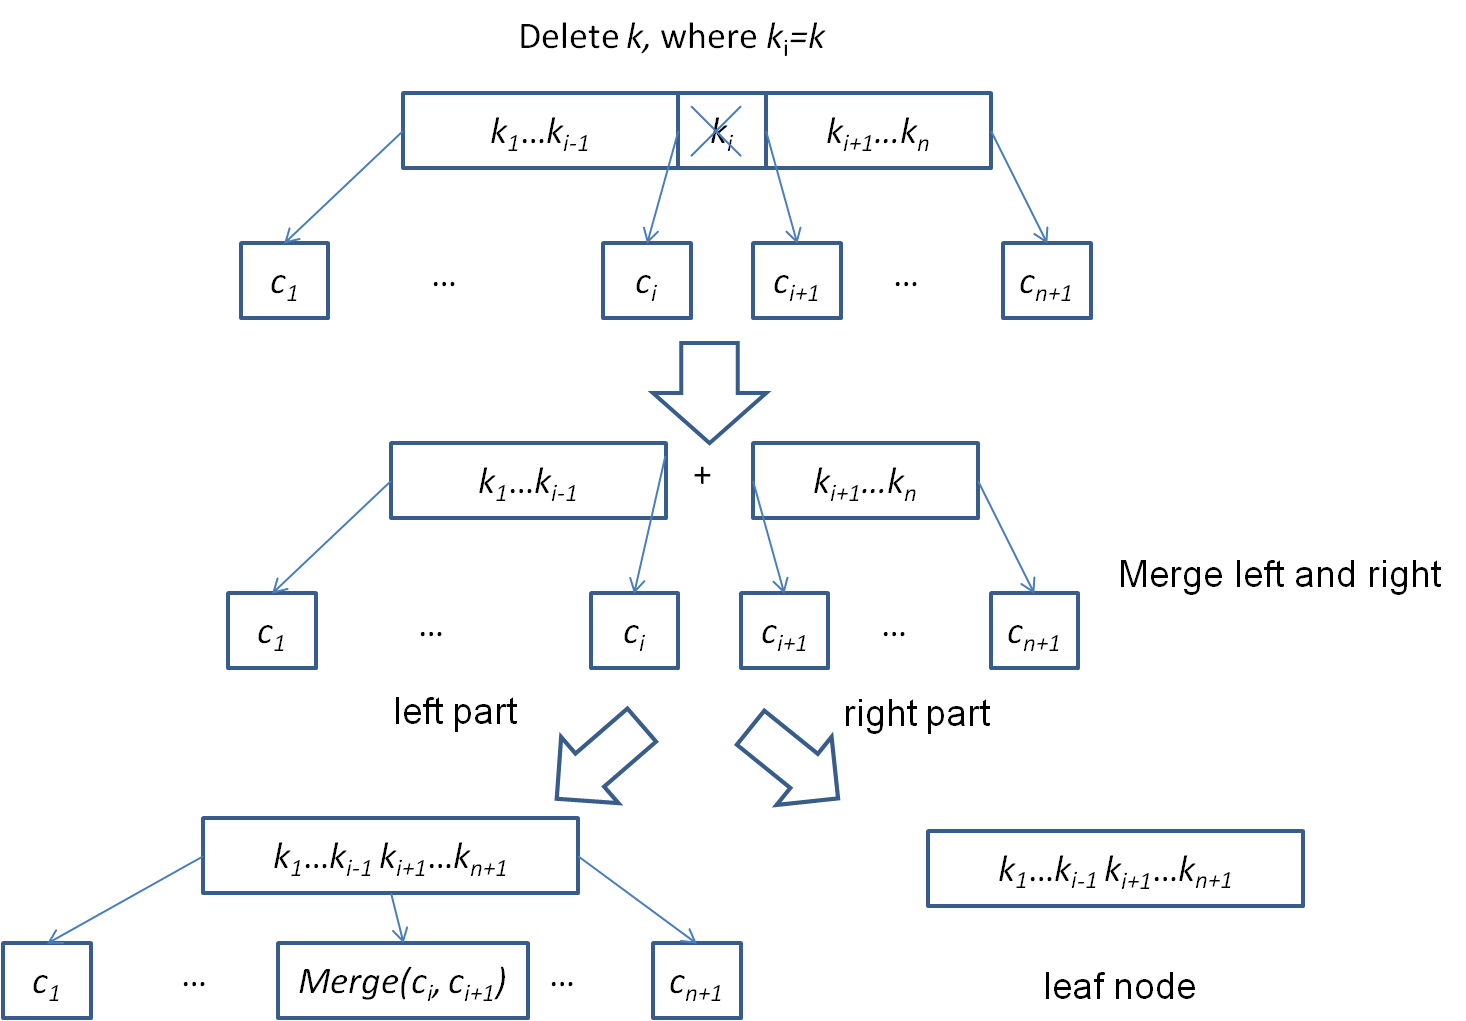
\includegraphics[scale=0.5]{img/btree-del-fp-merge.eps}
  \caption{Delete a key from a branch node. Removing $k_i$ breaks
the node into 2 parts. Merging these 2 parts
is a recursive process. When the two parts are leaves, the merging
terminates.} \label{fig:del-fp-merge}
\end{figure}

When do merging, if the two nodes are not leaves, we merge the keys
together, and recursively merge the last child of the left part
and the first child of the right part to one new node. Otherwise,
if they are leaves, we merely put all keys together.

Till now, the deleting is performed in straightforward way. However, deleting
decreases the number of keys of a node, and it may result in
violating the B-tree balance properties. The solution is to perform
fixing along the path traversed from root.

\begin{figure}[htbp]
  \centering
  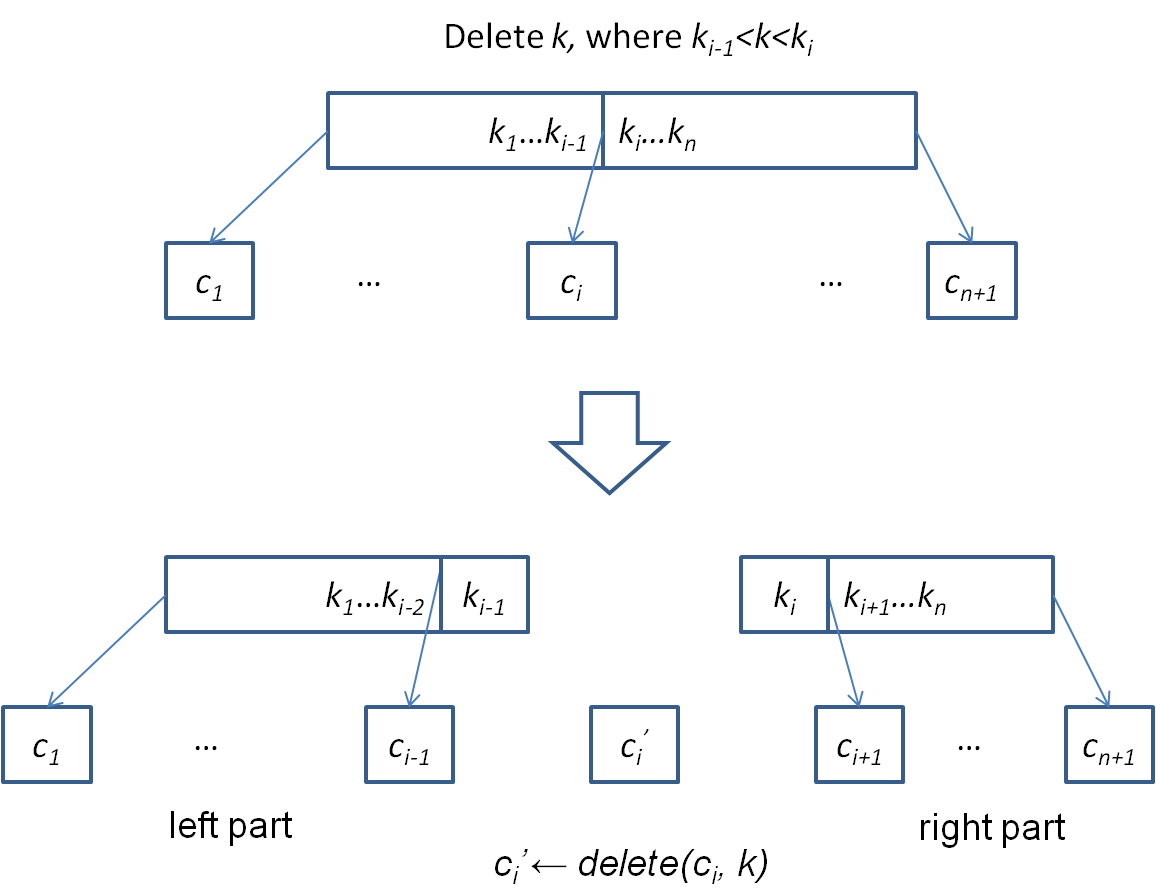
\includegraphics[scale=0.5]{img/btree-del-fp-make.eps}
  \caption{After delete key $k$ from node $c_i$, denote the result
as $c_i'$. The fixing makes a new node from the
left part, $c_i'$ and the right part.}
  \label{fig:del-fp-make}
\end{figure}

During the recursive deletion, the branch node is broken into 3 parts.
The left part contains all keys less than $k$, includes $k_1, k_2, ..., k_{i-1}$,
and children $c_1, c_2, ..., c_{i-1}$, the right part contains all keys
greater than $k$, say $k_i, k_{i+1}, ..., k_{n+1}$, and children
$c_{i+1}, c_{i+2}, ..., c_{n+1}$. Then key $k$ is recursively deleted
from child $c_i$. Denote the result becomes $c_i'$ after that.
We need make a new node from these 3 parts,
as shown in figure \ref{fig:del-fp-make}.

At this time point, we need examine if $c_i'$ contains enough keys.
If there are too less keys (less than $t-1$, but not $t$ in
contrast to the merge-and-delete approach), we can either borrow a key-child
pair from the left or the right part, and do inverse operation of
splitting. Figure \ref{fig:del-fp-fixlow} shows example of borrowing from the left part.

\begin{figure}[htbp]
  \centering
  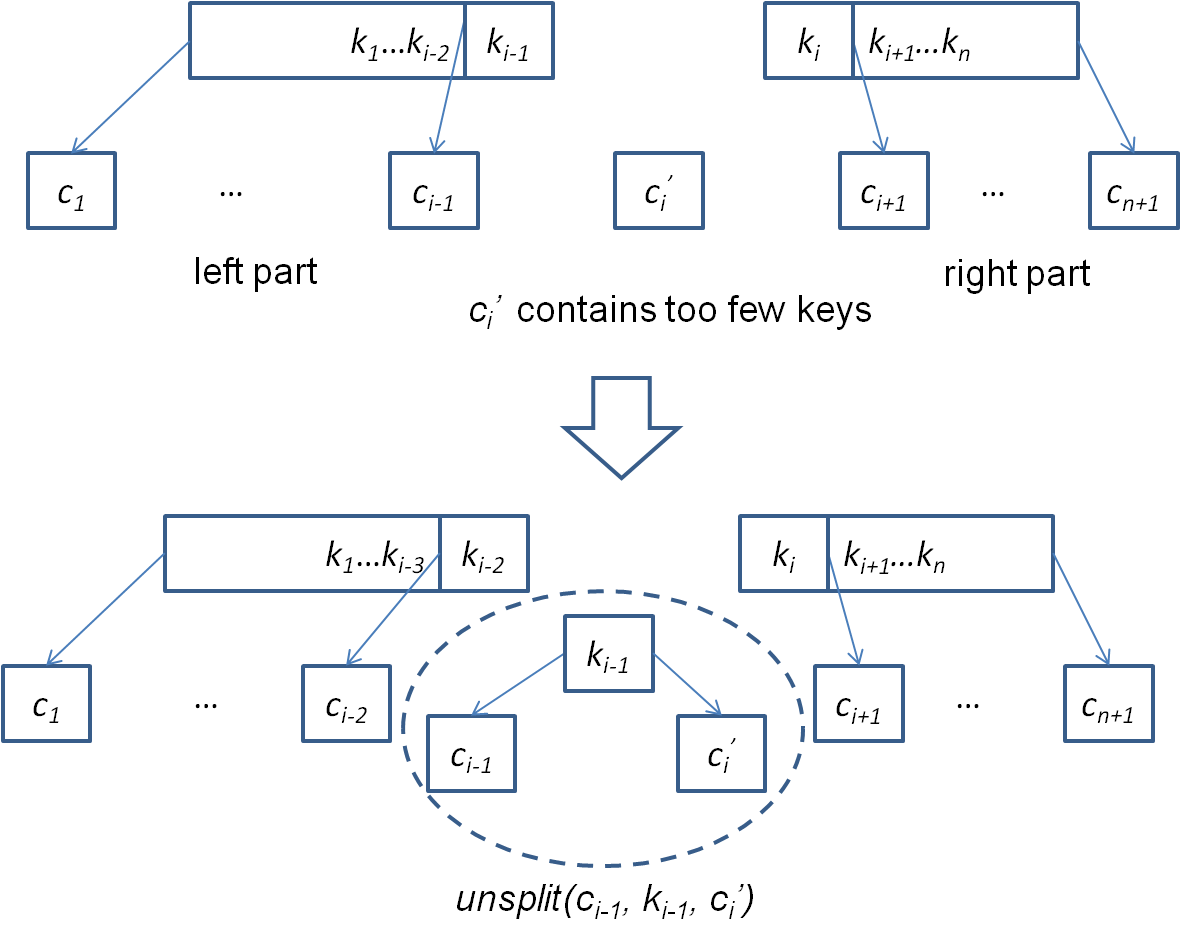
\includegraphics[scale=0.5]{img/btree-del-fp-fixlow.eps}
  \caption{Borrow a key-child pair from left part and
un-split to a new child.} \label{fig:del-fp-fixlow}
\end{figure}

If both left part and right part are empty, we can simply
push $c_i'$ up.

Denote the B-tree as $T=(K, C, t)$, where $K$ and $C$ are keys and children.
The $del(T, k)$ function deletes key $k$
from the tree.

\be
del(T, k) = \left \{
  \begin{array}
  {r@{\quad:\quad}l}
  (delete(K, k), \phi, t) & C = \phi \\
  merge((K_1, C_1, t), (K_2, C_2, t)) & k_i = k \\
  make((K_1', C_1'), del(c, k), (K_2', C_2')) & k \notin K
  \end{array}
\right.
\ee

If children $C = \phi$ is empty, $T$ is leaf. $k$ is deleted from keys directly.
Otherwise, $T$ is internal node. If $k \in K$, removing it separates the keys
and children in two parts $(K_1, C_1)$ and $(K_2, C_2)$. They will be recursively
merged.

\[
\begin{array}{l}
K_1 = \{k_1, k_2, ..., k_{i-1}\} \\
K_2 = \{k_{i+1}, k_{i+2}, ..., k_m\} \\
C_1 = \{c_1, c_2, ..., c_i\} \\
C_2 = \{c_{i+1}, c_{i+2}, ..., c_{m+1}\}
\end{array}
\]

If $k \notin K$, we need locate a child $c$, and further delete $k$ from
it.

\[
\begin{array}{l}
(K_1', K_2') = (\{k' | k' \in K, k' < k \}, \{k' | k' \in K, k < k' \}) \\
(C_1', \{c\} \cup C_2') = splitAt(|K_1'|, C)
\end{array}
\]

The recursive merge function is defined as the following. When merge two
trees $T_1 = (K_1, C_1, t)$ and $T_2 = (K_2, C_2, t)$, if both are leaves,
we create a new leave by concatenating the keys. Otherwise, the last
child in $C_1$, and the first child in $C_2$ are recursively merged.
And we call $make$ function to form the new tree. When $C_1$ and $C_2$
are not empty, denote the last child of $C_1$ as $c_{1, m}$, the rest
as $C_1'$; the first child of $C_2$ as $C_{2, 1}$, the rest as $C_2'$.
Below equation defines the merge function.

\be
merge(T_1, T_2) = \left \{
  \begin{array}
  {r@{\quad:\quad}l}
  (K_1 \cup K_2, \phi, t) & C_1 = C_2 = \phi \\
  make((K_1, C_1'), merge(c_{1,m}, c_{2, 1}), (K_2, C_2')) & otherwise
  \end{array}
\right.
\ee

The $make$ function defined above only handles the case that a node
contains too many keys due to insertion. When delete key, it may
cause a node contains too few keys. We need test and fix this
situation as well.

\be
make((K', C'), c, (K'', C'')) = \left \{
  \begin{array}
  {r@{\quad:\quad}l}
  fixFull((K', C'), c, (K'', C'')) & full(c) \\
  fixLow((K', C'), c, (K'', C'')) & low(c) \\
  (K' \cup K'', C' \cup \{c\} \cup C'', t) & otherwise
  \end{array}
\right.
\ee

Where $low(T)$ checks if there are too few keys less than $t-1$.
Function $fixLow(P_l, c, P_r)$ takes three arguments, the left pair of keys and children,
a child node, and the right pair of keys and children.
If the left part isn't empty, we borrow a pair of key-child, and
do un-splitting to make the child contain enough keys, then recursively
call $make$; If the right part isn't empty, we borrow a pair
from the right; and if both sides are empty, we
return the child node as result. In this case, the height of the tree
shrinks.

Denote the left part $P_l = (K_l, C_l)$. If $K_l$ isn't empty, the last
key and child are represented as $k_{l, m}$ and $c_{l, m}$ respectively.
The rest keys and children become $K_l'$ and $C_l'$; Similarly, the
right part is denoted as $P_r = (K_r, C_r)$. If $K_r$ isn't empty, the
first key and child are represented as $k_{r, 1}$, and $c_{r, 1}$. The
rest keys and children are $K_r'$ and $C_r'$. Below equation gives
the definition of $fixLow$.

\be
fixLow(P_l, c, P_r) = \left \{
  \begin{array}
  {r@{\quad:\quad}l}
  make((K_l', C_l'), unsplit(c_{l, m}, k_{l, m}, c), (K_r, C_r)) & K_l \neq \phi \\
  make((K_r, C_r), unsplit(c, k_{r, 1}, c_{r, 1}), (K_r', C_r')) & K_r \neq \phi \\
  c & otherwise
  \end{array}
\right.
\ee

Function $unsplit(T_1, k, T_2)$ is the inverse operation to splitting.
It forms a new B-tree nodes from two small nodes and a key.

\be
unsplit(T_1, k, T_2) = (K_1 \cup \{k\} \cup K_2, C_1 \cup C_2, t)
\ee

The following example Haskell program implements the B-tree deletion
algorithm.

\lstset{language=Haskell}
\begin{lstlisting}
import qualified Data.List as L

delete tr x = fixRoot $ del tr x

del:: (Ord a) => BTree a -> a -> BTree a
del (Node ks [] t) x = Node (L.delete x ks) [] t
del (Node ks cs t) x =
    case L.elemIndex x ks of
      Just i -> merge (Node (take i ks) (take (i+1) cs) t)
                      (Node (drop (i+1) ks) (drop (i+1) cs) t)
      Nothing -> make (ks', cs') (del c x) (ks'', cs'')
    where
      (ks', ks'') = L.partition (<x) ks
      (cs', (c:cs'')) = L.splitAt (length ks') cs

merge (Node ks [] t) (Node ks' [] _) = Node (ks++ks') [] t
merge (Node ks cs t) (Node ks' cs' _) = make (ks, init cs)
                                             (merge (last cs) (head cs'))
                                             (ks', tail cs')

make (ks', cs') c (ks'', cs'')
    | full c = fixFull (ks', cs') c (ks'', cs'')
    | low c  = fixLow  (ks', cs') c (ks'', cs'')
    | otherwise = Node (ks'++ks'') (cs'++[c]++cs'') (degree c)

low tr = (length $ keys tr) < (degree tr)-1

fixLow (ks'@(_:_), cs') c (ks'', cs'') = make (init ks', init cs')
                                              (unsplit (last cs') (last ks') c)
                                              (ks'', cs'')
fixLow (ks', cs') c (ks''@(_:_), cs'') = make (ks', cs')
                                              (unsplit c (head ks'') (head cs''))
                                              (tail ks'', tail cs'')
fixLow _ c _ = c

unsplit c1 k c2 = Node ((keys c1)++[k]++(keys c2))
                       ((children c1)++(children c2)) (degree c1)
\end{lstlisting}

When delete the same keys from the B-tree as in delete and fixing
approach, the results are different. However, both satisfy
the B-tree properties, so they are all valid.

\begin{figure}[htbp]
  \centering
  \subfloat[B-tree before deleting]{\includegraphics[scale=0.5]{img/btree-del-fp-before.ps}}\\
  \subfloat[After delete key 'E'.]{\includegraphics[scale=0.5]{img/btree-del-fp-E.ps}}
  \caption{Result of delete-then-fixing (1)} \label{fig:result-del-fp1}
\end{figure}

\begin{figure}[htbp]
  \centering
  \subfloat[After delete key 'G',]{\includegraphics[scale=0.5]{img/btree-del-fp-G.ps}} \\
  \subfloat[After delete key 'A'.]{\includegraphics[scale=0.5]{img/btree-del-fp-A.ps}}
  \caption{Result of delete-then-fixing (2)} \label{fig:result-del-fp2}
\end{figure}

\begin{figure}[htbp]
  \centering
  \subfloat[After delete key 'M'.]{\includegraphics[scale=0.5]{img/btree-del-fp-M.ps}} \\
  \subfloat[After delete key 'U'.]{\includegraphics[scale=0.5]{img/btree-del-fp-U.ps}}
  \caption{Result of delete-then-fixing (3)} \label{fig:result-del-fp3}
\end{figure}


% ================================================================
%               Searching
% ================================================================
\section{Searching}
\index{B-tree!search}

Searching in B-tree can be considered as the generalized
tree search extended from binary search tree.

When searching in the binary tree, there are only 2 different directions,
the left and the right. However, there are multiple directions in B-tree.

\begin{algorithmic}[1]
\Function{Search}{$T, k$}
  \Loop
    \State $i \gets 1$
    \While{$i \leq |K(T)| \land k > k_i(T)$}
      \State $i \gets i+1$
    \EndWhile
    \If{$i \leq |K(T)| \land k = k_i(T)$}
      \State \Return $(T, i)$
    \EndIf
    \If{$T$ is leaf}
      \State \Return $NIL$ \Comment{$k$ doesn't exist}
    \Else
      \State $T \gets c_i(T)$
    \EndIf
  \EndLoop
\EndFunction
\end{algorithmic}

Starts from the root, this program examines each key one by one
from the smallest to the biggest. In case it finds the
matched key, it returns the current node and the index of this
key. Otherwise, if it finds the position $i$ that $k_i < k < k_{i+1}$,
the program will next search the child node
$c_{i+1}$ for the key. If it traverses to some leaf node, and
fails to find the key, the empty value is returned to
indicate that this key doesn't exist in the tree.

The following example Python program implements the search algorithm.

\lstset{language=Python}
\begin{lstlisting}
def B_tree_search(tr, key):
    while True:
        for i in range(len(tr.keys)):
            if key <= tr.keys[i]:
                break
        if key == tr.keys[i]:
            return (tr, i)
        if tr.leaf:
            return None
        else:
            if key > tr.keys[-1]:
                i=i+1
            tr = tr.children[i]
\end{lstlisting}

The search algorithm can also be realized by recursion. When search
key $k$ in B-tree $T = (K, C, t)$, we partition the keys with $k$.

\[
\begin{array}{l}
K_1 = \{ k' | k' < k \} \\
K_2 = \{ k' | k \leq k' \}
\end{array}
\]

Thus $K_1$ contains all the keys less than $k$, and $K_2$ holds the
rest. If the first element in $K_2$ is equal to $k$, we find the key.
Otherwise, we recursively search the key in child $c_{|K_1|+1}$.

\be
search(T, k) = \left \{
  \begin{array}
  {r@{\quad:\quad}l}
  (T, |K_1|+1) & k \in K_2 \\
  \phi & C = \phi \\
  search(c_{|K_1|+1}, k) & otherwise
  \end{array}
\right.
\ee

Below example Haskell program implements this algorithm.

\lstset{language=Haskell}
\begin{lstlisting}
search :: (Ord a)=> BTree a -> a -> Maybe (BTree a, Int)
search tr@(Node ks cs _) k
    | matchFirst k $ drop len ks = Just (tr, len)
    | otherwise = if null cs then Nothing
                  else search (cs !! len) k
    where
      matchFirst x (y:_) = x==y
      matchFirst x _ = False
      len = length $ filter (<k) ks
\end{lstlisting}


% ================================================================
%                 Short summary
% ================================================================
\section{Notes and short summary}
In this chapter, we explained the B-tree data structure as a kind of
extension from binary search tree. The background knowledge of
magnetic disk access is skipped, user can refer to \cite{CLRS}
for detail. For the three main operations, insertion, deletion,
and searching, both imperative and functional algorithms are
given. They traverse from the root to the leaf. All the three
operations perform in time proportion to the height of the tree.
Because B-tree always maintains the balance properties. The
performance is ensured to bound to $O(\lg n)$ time,
where $n$ is the number of the keys in B-tree.

\begin{Exercise}
\begin{itemize}
\item When insert a key, we need find a position, where all keys on the left are less than it, while all the others on the right are greater than it. Modify the algorithm so that the elements stored in B-tree only need support less-than and equality test.
\item We assume the element being inserted doesn't exist in the tree. Modify the algorithm so that duplicated elements can be stored in a linked-list.
\item Eliminate the recursion in imperative B-tree insertion algorithm.
\end{itemize}
\end{Exercise}

\begin{thebibliography}{99}

\bibitem{CLRS}
Thomas H. Cormen, Charles E. Leiserson, Ronald L. Rivest and Clifford Stein. ``Introduction to Algorithms, Second Edition''. The MIT Press, 2001. ISBN: 0262032937.

\bibitem{wiki-b-tree}
B-tree, Wikipedia. http://en.wikipedia.org/wiki/B-tree

\bibitem{okasaki-rbtree}
Chris Okasaki. ``FUNCTIONAL PEARLS Red-Black Trees in a Functional Setting''. J. Functional Programming. 1998

\end{thebibliography}

\ifx\wholebook\relax \else
\end{document}
\fi
